60. $\cfrac{(y^2-4)(y+2x-1)}{x-1}=0\Leftrightarrow\cfrac{(y-2)(y+2)(y-(1-2x))}{x-1}=0\Leftrightarrow\begin{cases}
\left[\begin{array}{l} y=2,\\ y=-2, \\ y=1-2x.\end{array}
ight.\\ x
eq1.\end{cases}$
$$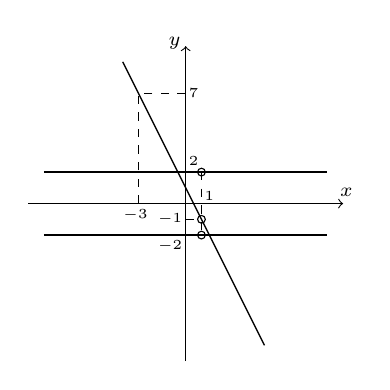
\begin{tikzpicture}[scale=0.2]
\tikzset {line01/.style={line width =0.5pt}}
\tikzset{line02/.style={line width =1pt}}
\tikzset{line03/.style={dashed,line width =0.5pt}}
%\filldraw [black] (0,0) circle (1pt);
\draw [->] (-10,0) -- (10,0);
\draw [->] (0,-10) -- (0,10);
\draw[line01] (-9,2) -- (9,2);
\draw[line01] (-9,-2) -- (9,-2);
\draw[line01] (5,-9) -- (-4,9);
\draw[line03] (1,2) -- (1,-2);
\draw[line03] (0,-1) -- (1,-1);
\draw[line03] (-3,0) -- (-3,7);
\draw[line03] (0,7) -- (-3,7);
\draw (1.5,0.5) node {\tiny $1$};
\draw (-3.2,-0.7) node {\tiny $-3$};
\draw (0.5,7) node {\tiny $7$};
\draw (0.5,2.7) node {\tiny $2$};
\draw (-1,-2.7) node {\tiny $-2$};
\draw (-1,-1) node {\tiny $-1$};
\draw (10.2,0.7) node {\scriptsize $x$};
\draw (-0.7,10.2) node {\scriptsize $y$};
\draw (1,2) circle (7pt);
\draw (1,-2) circle (7pt);
\draw (1,-1) circle (7pt);
\end{tikzpicture}$$
